%\Blindtext
%\lipsum[1-3]
%\vspace{2cm} % Add 2 cm of vertical space here

%---- jonswap, ikke direkte en del av oppgaven.
\section{JONSWAP}
The standard deviation of the response, in an irregular sea given by a spectrum, S(omega),
may be expressed by
\begin{align}
\sigma_r^2 = \int_0^{\infty} S(\omega) \left|\frac{\xi_2}{A}\right|^2d\omega
\end{align}

where a calculation (script below) using the functions in figure 11, with T = 6 seconds
and D = 15 m (and L/D = 2) gives sigmar simeq 0.358H1/3. This means that if H1/3 = 8 m the
standard deviation of the heave response is sigmar simeq 2.86 m.


%------

\section{}
vi ønsker å løse integrallikningen:
\begin{equation}
    -\pi \phi(\bar{x}\bar{y})  + \int_{S} \phi  \frac{\partial }{\partial n} \ln r dS = \int_{S}  \frac{\partial \phi}{\partial n} \ln r dS
\end{equation}
der $\partial \phi / \partial n = n_1$ langs med S.

Diskret integrallikning.
\begin{equation}
    -\pi \phi  + \Sigma_{m=1}^N \phi_m (-\Delta \Theta_{n,m})   =  \sum_{m=1}^N [\frac{\partial \phi}{\partial n}]_m h_{n,m}
\end{equation}

Addert masse kan approksimeres slik:
\begin{equation}
    m_{ij}  = \rho \int_{S} \phi_j n_i dS \, \simeq \, \rho \sum_{m=1}^N [\phi_j]_m  [n_i]_m \Delta S_m.
\end{equation}


\section{Figurer}
\subsection{Diskretisering av boks}


{\noindent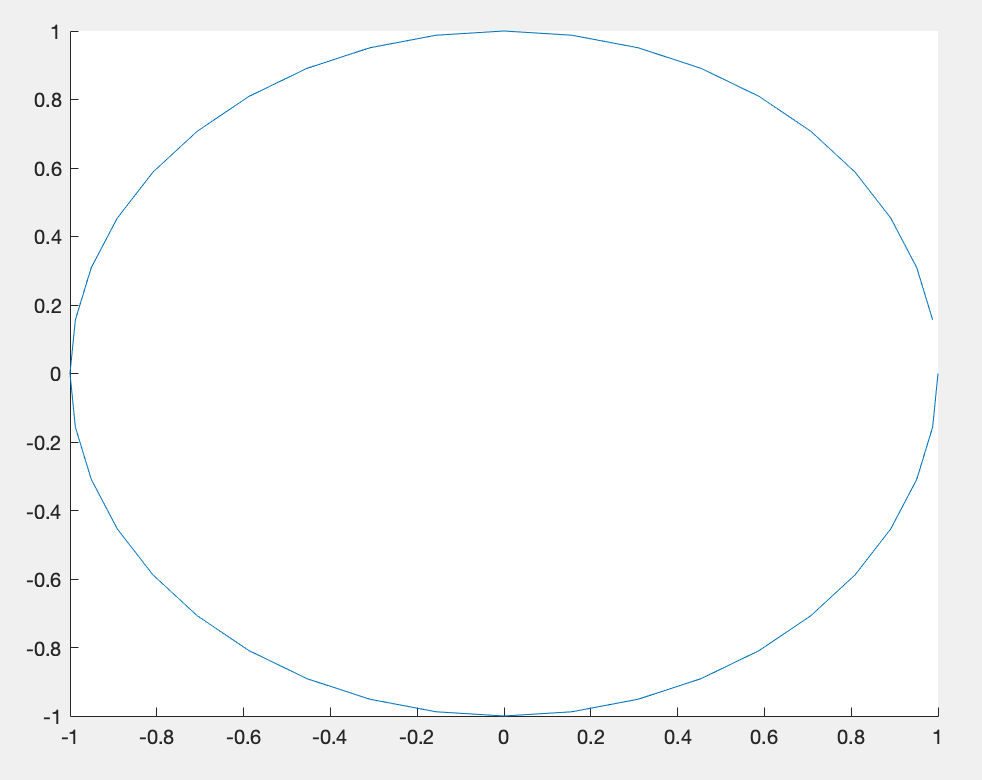
\includegraphics[width=\linewidth]{/Users/ole/Tex/MEK4420/oblig2images/placeholder.png}
\captionof{figure}{}}

\subsection{7.8}

\begin{align}
	b_{22} &=  \frac{\bar{E}^{\infty} c_g + \bar{E}^{-\infty} c_g }{\frac{1}{2} |\xi|^2 \omega^2}\\
	b_{22} &=  \frac{\frac{1}{2}\rho g |amp^{-\infty}|^2  c_g + \frac{1}{2}\rho g |amp^{-\infty}|^2 c_g }{\frac{1}{2} |\xi|^2 \omega^2}\\
	b_{22} &=  \frac{\frac{1}{2}\rho g |amp^{-\infty}|^2  (\frac{g}{2\omega}) + \frac{1}{2}\rho g |amp^{-\infty}|^2 (\frac{g}{2\omega}) }{\frac{1}{2} |\xi|^2 \omega^2}\\
	b_{22} &=  \frac{\frac{1}{2}\rho g {|\xi A^{\infty} \frac{\omega^2}{g}|}^2  (\frac{g}{2\omega}) + \frac{1}{2}\rho g {|\xi A^{-\infty} \frac{\omega^2}{g}|}^2  (\frac{g}{2\omega}) }{\frac{1}{2} |\xi|^2 \omega^2}\\
	b_{22} &=  \frac{\frac{1}{2}\rho g {|\xi A^{\infty} \frac{\omega^2}{g}|}^2  (\frac{g}{2\omega}) + \frac{1}{2}\rho g {|\xi A^{-\infty} \frac{\omega^2}{g}|}^2  (\frac{g}{2\omega}) }{\frac{1}{2} |\xi|^2 \omega^2}\\
b_{22} &=  \frac{\frac{1}{2}\rho g |\xi|^2 (\frac{\omega^2}{g})^2 {| A^{\infty} |}^2  (\frac{g}{2\omega}) + \frac{1}{2}\rho g |\xi|^2  (\frac{\omega^2}{g})^2 {| A^{-\infty}|}^2  (\frac{g}{2\omega}) }{\frac{1}{2} |\xi|^2 \omega^2}\\
b_{22} &=  \frac{\frac{1}{2}\rho g |\xi|^2 (\frac{\omega^2}{g})(\frac{\omega^2}{g}) {| A^{\infty} |}^2  (\frac{g}{2\omega}) + \frac{1}{2}\rho g |\xi|^2  (\frac{\omega^2}{g})(\frac{\omega^2}{g}) {| A^{-\infty}|}^2  (\frac{g}{2\omega}) }{\frac{1}{2} |\xi|^2 \omega^2}\\
b_{22} &=  \frac{ \cancel{\frac{1}{2}}\rho g \cancel{|\xi|^2} (\frac{\color{red}{\omega^2}}{g})(\frac{\omega^2}{g}) {| A^{\infty} |}^2  (\frac{g}{2\omega}) + \cancel{\frac{1}{2}}\rho g \cancel{|\xi|^2}  (\frac{\color{red}{\omega^2}}{g})(\frac{\omega^2}{g}) {| A^{-\infty}|}^2  (\frac{g}{2\omega}) }{\cancel{\frac{1}{2}} \cancel{|\xi|^2} \color{red}{\omega^2}}\\
b_{22} &=   \rho \cancel{g  (\frac{1}{g})}(\frac{\omega^2}{g}) {| A^{\infty} |}^2  (\frac{g}{2\omega}) + \rho \cancel{g   (\frac{1}{g})}(\frac{\omega^2}{g}) {| A^{-\infty}|}^2  (\frac{g}{2\omega}) \\
\end{align}

\[
\cancelto{D} + \color{red} + \color{blue}\cancel{22}  \color{green}00
\]
